\documentclass[tikz,border=12pt]{standalone}
\usepackage{amsmath,amssymb}
\usepackage{tikz}
\usetikzlibrary{arrows.meta,positioning,calc}

\definecolor{dqC}{HTML}{0B6E4F}
\definecolor{modC}{HTML}{5B2C6F}
\definecolor{ink}{HTML}{1A1A1A}
\definecolor{bgSoft}{HTML}{F7F5F1}

\begin{document}
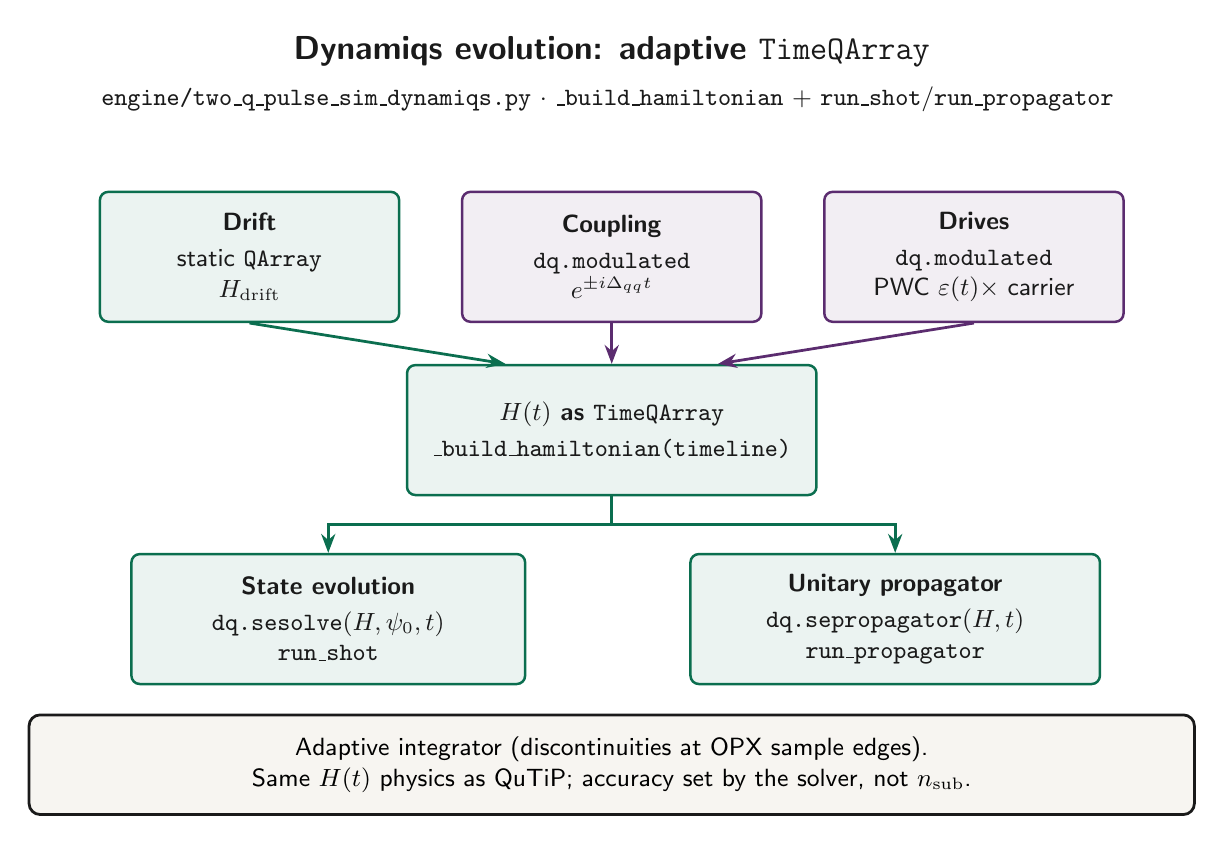
\begin{tikzpicture}[
  font=\sffamily\small,
  >={Stealth[length=2.4mm]},
  box/.style={
    draw=#1, line width=0.9pt, rounded corners=3pt,
    fill=#1!8, align=center, inner sep=7pt, text=ink,
    minimum width=3.8cm, minimum height=1.65cm
  },
  title/.style={font=\sffamily\bfseries\large, text=ink}
]

\node[title] at (0,5.15) {Dynamiqs evolution: adaptive \texttt{TimeQArray}};
\node[align=center, text=ink] at (0,4.55) {%
  \texttt{engine/two\_q\_pulse\_sim\_dynamiqs.py} $\cdot$
  \texttt{\_build\_hamiltonian} + \texttt{run\_shot}/\texttt{run\_propagator}
};

% evenly spaced inputs
\node[box=dqC] (D) at (-4.6,2.55) {%
  \textbf{Drift}\\[2pt]
  static \texttt{QArray}\\
  $H_{\mathrm{drift}}$
};

\node[box=modC] (C) at (0,2.55) {%
  \textbf{Coupling}\\[2pt]
  \texttt{dq.modulated}\\
  $e^{\pm i\Delta_{qq}t}$
};

\node[box=modC] (R) at (4.6,2.55) {%
  \textbf{Drives}\\[2pt]
  \texttt{dq.modulated}\\
  PWC $\varepsilon(t)\times$ carrier
};

\node[box=dqC, minimum width=5.2cm] (H) at (0,0.35) {%
  \textbf{$H(t)$ as \texttt{TimeQArray}}\\[2pt]
  \texttt{\_build\_hamiltonian(timeline)}
};

% three independent downward arrows into H
\draw[->, line width=1pt, dqC]  (D.south) -- ([xshift=-1.35cm]H.north);
\draw[->, line width=1pt, modC] (C.south) -- (H.north);
\draw[->, line width=1pt, modC] (R.south) -- ([xshift=1.35cm]H.north);

\node[box=dqC, minimum width=5.0cm] (S) at (-3.6,-2.05) {%
  \textbf{State evolution}\\[2pt]
  \texttt{dq.sesolve}$(H,\psi_0,t)$\\
  \texttt{run\_shot}
};

\node[box=dqC, minimum width=5.2cm] (U) at (3.6,-2.05) {%
  \textbf{Unitary propagator}\\[2pt]
  \texttt{dq.sepropagator}$(H,t)$\\
  \texttt{run\_propagator}
};

% fork from H into the two solvers
\coordinate (fork) at (0,-0.85);
\draw[line width=1pt, dqC] (H.south) -- (fork);
\draw[->, line width=1pt, dqC] (fork) -| (S.north);
\draw[->, line width=1pt, dqC] (fork) -| (U.north);

\node[draw=ink, line width=1pt, rounded corners=4pt, fill=bgSoft,
      align=center, inner sep=8pt, minimum width=14.8cm]
  at (0,-3.9) {%
  Adaptive integrator (discontinuities at OPX sample edges).\\
  Same $H(t)$ physics as QuTiP; accuracy set by the solver, not $n_{\mathrm{sub}}$.
};

\end{tikzpicture}
\end{document}
